%
% Copyright 2018 Joel Feldman, Andrew Rechnitzer and Elyse Yeager.
% This work is licensed under a Creative Commons Attribution-NonCommercial-ShareAlike 4.0 International License.
% https://creativecommons.org/licenses/by-nc-sa/4.0/
%
\questionheader{ex:s3.5.3}
%%%%%%%%%%%%%%%%%%
\subsection*{\Procedural}
%%%%%%%%%%%%%%%%%%
\Instructions{For Questions~
\ref{s3.5.3given1} through
\ref{s3.5.3given3}, the quantity to optimize is already given to you as a function of a single variable.}

\begin{question}[2015Q]\label{s3.5.3given1}
Find the global maximum and the global minimum for $f(x)=x^5 - 5x + 2$ on the interval $[-2,0]$.
\end{question}
\begin{hint}
Factor the derivative.
\end{hint}
\begin{answer}
The global maximum is $f(-1) = 6$, the global minimum is $f(-2) = -20$.
\end{answer}
\begin{solution}
We compute $f'(x)=5\,x^4 - 5$, which means that $f(x)$ has no singular points (i.e., it is
differentiable for all values of $x$), but it has two critical points:
\begin{align*}
0&=5x^4-5\\
0&=x^4-1=(x^2+1)(x^2-1)\\
0&=x^2-1\\
x&= \pm 1
\end{align*}
Note, however, that $1$ is not in the interval $[-2,0]$.

The global maximum and the
global minimum for $f(x)$ on the interval $[-2,0]$ will occur at $x=-2$, $x=0$, or $x=-1$.
\begin{center}
\begin{tabular}{|c||c|c|c|}
\hline
$c$ & $-2$ &  $0$ &  $-1$  \\
\hline
type & endpoint & endpoint & critical point  \\
\hline
$f(c)$ & $-20$ & $2$ & $6$ \\
\hline
\end{tabular}
\end{center}

So, the global maximum is $f(-1) = 6$ while the global minimum is $f(-2) = -20$.
\end{solution}



\begin{question}[2015Q]
Find the global maximum and the global minimum for $f(x)=x^5 - 5x - 10$ on the interval $[0,2]$.
\end{question}
\begin{hint} Remember to test endpoints.
\end{hint}
\begin{answer} Global maximum is $f(2) = 12$, global minimum is $f(1) = -14$.
\end{answer}
\begin{solution} We compute $f'(x)=5x^4-5$, which means that $f(x)$ has no singular points (i.e., it is differentiable for all values of $x$), but it has two critical points:
\begin{align*}
0&=5x^4-5\\
0&=x^4-1=(x^2+1)(x^2-1)\\
0&=x^2-1\\
x&= \pm 1
\end{align*}
Note, however, that $-1$ is not in the interval $[0,2]$.

The global maximum and the
global minimum for $f(x)$ on the interval $[0,2]$ will occur at $x=2$, $x=0$, or $x=1$.
\begin{center}
\begin{tabular}{|c||c|c|c|}
\hline
$c$ & $2$ &  $0$ &  $1$  \\
\hline
type & endpoint & endpoint & critical point  \\
\hline
$f(c)$ & $12$ & $-10$ & $-14$ \\
\hline
\end{tabular}
\end{center}

So, the global maximum is $f(2) = 12$ while the global minimum is $f(1) = -14$.
\end{solution}


\begin{question}[2015Q]\label{s3.5.3given3}
Find the global maximum and the global minimum for $f(x)=2x^3 - 6x^2 - 2$ on the interval $[1,4]$.
\end{question}
\begin{answer}
Global maximum is $f(4) = 30$, global minimum is $f(2) = -10$.
\end{answer}
\begin{solution}
We compute $f'(x)=6x^2 - 12x = 6x(x-2)$, which means that $f(x)$ has no singular points
(i.e., it is differentiable for all values of $x$), but it has the two critical points:
$x=0$ and $x=2$.
Note, however, $0$ is not in the interval $[1,4]$.
\begin{center}
\begin{tabular}{|c||c|c|c|}
\hline
$c$ & $1$ &  $4$ &  $2$  \\
\hline
type & endpoint & endpoint & critical point  \\
\hline
$f(c)$ & $-6$ & $30$ & $-10$ \\
\hline
\end{tabular}
\end{center}

So, the global maximum is $f(4) = 30$ while the global minimum is $f(2) = -10$.
\end{solution}


\Instructions{For Questions~\ref{s3.5.3firstderivfirst} and \ref{s3.5.3firstderivlast}, you  can decide whether a critical point is a local extrema by considering the derivative of the function.}

\begin{Mquestion}[2015Q]\label{s3.5.3firstderivfirst}
Consider the function $h(x)=x^3-12x+4$.
What are the coordinates of the local maximum of $h(x)$? What are the coordinates of the local minimum of $h(x)$?
\end{Mquestion}
\begin{hint}
One way to decide whether a critical point $x=c$ is a local extremum is to consider the first derivative. For example: if $f'(x)$ is negative for all $x$ just to the left of $c$, and positive for all $x$ just to the right of $c$, then $f(x)$ decreases up till $c$, then increases after $c$, so $f(x)$ has a local minimum at $c$.
\end{hint}
\begin{answer} Local max at $(-2,20)$, local min at $(2,-12)$.
\end{answer}
\begin{solution}
Since $h(x)$ is a polynomial, it has no singular points. We compute its critical points:
\begin{align*}
h'(x)&=3x^2-12\\
0&=3x^2-12\\
x&=\pm 2
\end{align*}
Notice as $x\to\infty$, $h(x)\to\infty$, and as $x\to-\infty$ $h(x)\to-\infty$. So Theorem~\ref*{thm:maxMinOnR} doesn't exactly apply. Instead, let's consider the signs of $h'(x)$.

\begin{center}
\begin{tabular}{|c||c|c|c|}
\hline
$x$ & $(-\infty,-2)$ &  $(-2,2)$ &  $(2,\infty)$  \\
\hline
$h'(x)$ & $>0$ & $<0$ & $>0$ \\
\hline
$h(x)$ & increasing & decreasing & increasing  \\
\hline
\end{tabular}
\end{center}
So, $h(x)$ increases until $x=-2$, then decreases. That means $h(x)$ has a local maximum at $x=-2$. The function decreases from $-2$ until $2$, after which is increases, so $h(x)$ has a local minimum at $x=2$.
We compute $f(-2)=20$ and $f(2)=-12$.
\end{solution}



\begin{question}[2015Q]\label{s3.5.3firstderivlast}
Consider the function $h(x)=2x^3-24x+1$.
What are the coordinates of the local maximum of $h(x)$? What are the coordinates of the local minimum of $h(x)$?
\end{question}
\begin{hint}
One way to decide whether a critical point $x=c$ is a local extremum is to consider the first derivative. For example: if $f'(x)$ is negative for all $x$ just to the left of $c$, and positive for all $x$ just to the right of $c$, then $f(x)$ decreases up till $c$, then increases after $c$, so $f(x)$ has a local minimum at $c$.
\end{hint}
\begin{answer}
$(-2,33)$ max, and $(2,-31)$ min
\end{answer}
\begin{solution}
Since $h(x)$ is a polynomial, it has no singular points. We compute its critical points:
\begin{align*}
h'(x)&=6x^2-24\\
0&=6x^2-24\\
x&=\pm2
\end{align*}
Notice as $x\to\infty$, $h(x)\to\infty$, and as $x\to-\infty$ $h(x)\to-\infty$. So Theorem~\ref*{thm:maxMinOnR} doesn't exactly apply. Instead, let's consider the signs of $h'(x)$.

\begin{center}
\begin{tabular}{|c||c|c|c|}
\hline
$x$ & $(-\infty,-2)$ &  $(-2,2)$ &  $(2,\infty)$  \\
\hline
$h'(x)$ & $>0$ & $<0$ & $>0$ \\
\hline
$h(x)$ & increasing & decreasing & increasing  \\
\hline
\end{tabular}
\end{center}
So, $h(x)$ increases until $x=-2$, then decreases. That means $h(x)$ has a local maximum at $x=-2$. The function decreases from $-2$ until $2$, after which is increases, so $h(x)$ has a local minimum at $x=2$.

 We compute $f(-2)=33$ and $f(2)=-31$.
\end{solution}


\Instructions{For Questions \ref{s3.5.3formulafirst} through \ref{s3.5.3formulalast}, you will have to find an expression for the quantity you want to optimize as a function of a single variable.}





\begin{Mquestion}[1999H, 2012H]\label{s3.5.3formulafirst}
You are in a dune buggy at a point $P$ in the desert, 12
km due south of the nearest point $A$ on a straight east-west road. You
want to get to a town $B$ on the road $18$ km east of $A$. If your dune
buggy can travel at an average speed of 15 km/hr through the desert and
30 km/hr along the road, towards what point $Q$ on the road should you
head to minimize your travel time from $P$ to $B$?

%\centerline{\figput{dune}}
\begin{center}
\begin{tikzpicture}
\draw[gray, line width=5pt, opacity=0.5] (-.5,3) -- (4.5,3);
\draw (0,3) node[vertex, label=above:$A$](A){};
\draw (3,3) node[vertex, label=above:$Q$](Q){};
\draw (4,3) node[vertex, label=above:$B$](B){};
\draw (0,0) node[vertex, label=left:$P$](P){};
\draw (A)--(P) node[midway, left]{12 km};
\draw[very thick] (P)--(Q)--(B);
\end{tikzpicture}
\end{center}
\end{Mquestion}
\begin{hint} Start with a formula for travel time from $P$ to $B$. You might want to assign a variable to the distance from $A$ where your buggy first reaches the road.
\end{hint}
\begin{answer} $Q$ should be $4\sqrt{3}$ kilometres from $A$
\end{answer}
\begin{solution}
Suppose that $Q$ is a distance of $x$ from $A$.
Then it is a distance of $18-x$ from $B$.
\begin{center}
\begin{tikzpicture}
\draw[gray, line width=5pt, opacity=0.5] (-.5,3) -- (4.5,3);
\draw (0,3) node[vertex, label=above:$A$](A){};
\draw (3,3) node[vertex, label=above:$Q$](Q){};
\draw (4,3) node[vertex, label=above:$B$](B){};
\draw (0,0) node[vertex, label=left:$P$](P){};
\draw (A)--(P) node[midway, left]{12 km};
\draw[very thick] (P)--(Q)--(B);
\draw[decorate, decoration={brace, amplitude=7pt}](0,3.75)--(3,3.75) node[midway, yshift=.5cm]{$x$};
\draw[decorate, decoration={brace, amplitude=7pt}](3,3.75)--(4,3.75) node[midway, yshift=.5cm]{$18-x$};
\end{tikzpicture}
\end{center}
Using the Pythagorean Theorem, the distance from $P$ to $Q$ is $\sqrt{12^2+x^2}$ kilometres, and the buggy travels 15 kph over this off-road stretch.
The travel time
from $P$ to $Q$ is $\dfrac{\sqrt{12^2+x^2}}{15}$ hours.

The distance from $Q$ to $B$ is $18-x$ kilometres, and the dune buggy travels $30$ kph along this road. The travel time from $Q$
to $B$ is $\dfrac{18-x}{30}$ hours.
So, the total travel time is
\[f(x)= \dfrac{\sqrt{12^2+x^2}}{15}+\dfrac{18-x}{30}.\] We wish to minimize
this for $0\le x\le 18$. We will test all singular points, critical points, and endpoints to find which yields the smallest value of $f(x)$. Since there are no singular points, we begin by locating the critical points.
\begin{align*}
0=f'(x)&=\dfrac{1}{15}\cdot\dfrac{1}{2}(144+x^2)^{-1/2}(2x)-\dfrac{1}{30}\\
\dfrac{1}{15}\cdot\dfrac{x}{\sqrt{144+x^2}}&=\dfrac{1}{30}\\
 \dfrac{x}{\sqrt{144+x^2}}&=\dfrac{1}{2}\\
 \dfrac{x^2}{144+x^2}&=\dfrac{1}{4}\\
 4x^2&=144+x^2\\
 x&=\dfrac{12}{\sqrt{3}}=4\sqrt{3}
\end{align*}
So the minimum travel times must be one of $f(0)$, $f(18)$, and $f\left(4\sqrt{3}\right)$.
\begin{align*}
f(0)&=\dfrac{12}{15}+\dfrac{18}{30}=1.4\cr
f(18)&=\dfrac{\sqrt{12^2+18^2}}{15}\approx1.44\cr
f\left({4\sqrt{3}}\right)&=
\dfrac{\sqrt{144+144/3}}{15}+\dfrac{18-12/\sqrt{3}}{30}
\approx1.29
\end{align*}
So $Q$ should be $4\sqrt{3}$ km from $A$.
\end{solution}

\begin{question}[1997D]
A closed three dimensional box is to be constructed in such
a way that its volume is 4500 cm${}^3$. It is also specified that the length
of the base is 3 times the width of the base. Find the dimensions of the
box that satisfies these conditions and has the minimum possible
surface area. Justify your answer.
\end{question}
\begin{hint}
A box has three dimensions; make variables for them, and write the relations given in the problem in terms of these variables.
\end{hint}
\begin{answer}
$10\times 30 \times 15$
\end{answer}
\begin{solution}
Let $\ell,\ w$ and $h$ denote the length, width and height
of the box respectively.
 We are told that $\ell w h =4500$ and that
$\ell=3w$. Hence $h=\dfrac{4500}{\ell w}=\dfrac{4500}{3 w^2}=\dfrac{1500}{w^2}$.
The surface area of the box is
$$
A=2\ell w+2\ell h+2 wh=2\left(3w^2+3w\dfrac{1500}{w^2}+w\dfrac{1500}{w^2}\right)
=2\left(3w^2+\dfrac{6000}{w}\right)=6\left(w^2+\dfrac{2000}{w}\right)
$$
\begin{center}
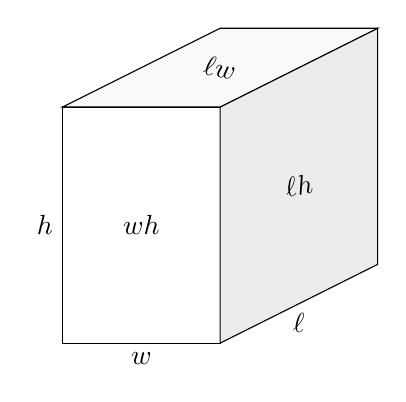
\begin{tikzpicture}
\draw (0,0) rectangle (2,3);
\draw[fill=gray!15] (2,3)--(4,4)--(4,1)--(2,0)--cycle;
\draw[fill=gray!5] (0,3)--(2,4)--(4,4)--(2,3)--cycle;
\draw (1,0) node[below]{$w$};
\draw (0,1.5) node[left]{$h$};
\draw (3,.5) node[below]{$\ell$};
\draw (1,1.5) node{$wh$};
\draw (2,3.5) node[rotate=-10]{$\ell w$};
\draw (3,2) node[rotate=10]{$\ell h$};
\end{tikzpicture}
\end{center}
As $w$ tends to zero or to infinity, the surface area approaches infinity.
By Theorem~\ref*{thm:maxMinOnR} the minimum surface area must occur at a critical point of
$w^2+\dfrac{2000}{w}$.
\begin{align*}
0&=\diff{}{w}\left\{w^2+\dfrac{2000}{w}\right\}\\
&=2w-\dfrac{2000}{w^2}\\
2w&=\dfrac{2000}{w^2}\\
w^3&=1000\hskip-3pt\\
 w&=10
 \intertext{Therefore,}
  \ell&=3w=30\\
   h&=\frac{1500}{w^2}=15.
\end{align*}
The dimensions of the box with minimum surface area are $10 \times 30 \times 15$.
\end{solution}






\begin{Mquestion}[1996D]
A closed rectangular container with a square base is to be made
from two different materials. The material for the base costs \$5 per square
metre, while the material for the other five sides costs \$1 per square
metre. Find the dimensions of the container which has the largest possible
volume if the total cost of materials is \$72.
\end{Mquestion}
\begin{hint} Find a formula for the cost of the base, and another formula for the cost of the other sides. The total cost is the sum of these two formulas.
\end{hint}
\begin{answer}
$2\times 2\times 6$
\end{answer}
\begin{solution}
Let the length of the sides of the square base be $b$ metres
and let the height be $h$ metres. The area of the base is $b^2$, the area
of the top is $b^2$  and the
area of each of the remaining four sides is $bh$ so the total cost is
\[
\underbrace{5(b^2)}_{\mbox{cost of base}}+\underbrace{1(b^2+4bh)}_{\mbox{cost of 5 sides}}=6b^2+4bh=72\]
{Solving for $h$,}
\begin{align*}
h&=\dfrac{72-6b^2}{4b}\\
&=\dfrac{6}{4}\left(\dfrac{12-b^2}{b}\right)\\
&=\dfrac{3}{2}\left(\dfrac{12-b^2}{b}\right)
\end{align*}
The volume is
\begin{align*}
V=b^2h&=b^2\cdot \dfrac{3}{2}\left(\dfrac{12-b^2}{b}\right)
\\
&=18b-\dfrac{3}{2}b^3.
\end{align*}
This is the function we want to maximize.
Since volume is never negative, the endpoints of the functions are the values of $b$ that make the volume 0. So, the maximum volume will not occur at an endpoint, it will occur at a critical point.
The only critical point is $b=2$:
\begin{align*}
0&=\diff{}{b}\left\{18b-\dfrac{3}{2}b^3\right\}\\
&=18-\dfrac{9}{2}b^2\\
 b^2&=4\\
  b&=2,\ h=\dfrac{3}{2}\left(\dfrac{12-4}{2}\right)=6
\end{align*}
The desired dimensions are $2\times 2\times 6$.
\end{solution}



\begin{question}[1998H]
Find a point $X$ on the positive $x$--axis and a point $Y$
on the positive $y$--axis such that (taking $O=(0,0)$)
\begin{enumerate}[(i)]
\item\label{s3.5inscribed1}The triangle $XOY$ contains the first quadrant portion of
the unit circle $x^2+y^2=1$ and
\item\label{s3.5inscribed2} the area of the triangle $XOY$ is as small as possible.
\end{enumerate}
A complete and careful mathematical justification of property \eqref{s3.5inscribed1}
is required.
\end{question}
\begin{hint}
The setup is this:
\begin{center}
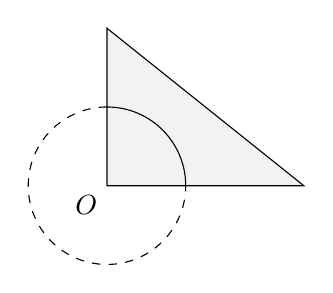
\begin{tikzpicture}
\YEaxis{3}{3}
\YExcoord{2.5}{X}
\YEycoord{2}{Y}
\draw (0,0) node[below left]{$O$};
\draw[fill=gray!10] (0,0)--(2.5,0)--(0,2)--cycle;
\draw (1,0) arc (0:90:1cm);
\draw[dashed] (0,1) arc(90:360:1cm);
\end{tikzpicture}
\end{center}
\end{hint}
\begin{answer}
$X=Y=\sqrt{2}$
\end{answer}
\begin{solution}
 It suffices to consider $X$ and $Y$ such that the line $XY$
is tangent to the circle. Otherwise we could reduce the area of the triangle
by, for example, holding $X$ fixed and reducing $Y$. So let $X$ and $Y$
be the $x$-- and $y$--intercepts of the line tangent to the circle at
$(\cos\theta,\sin\theta)$. Then $\dfrac{1}{X}=\cos\theta$ and
$\dfrac{1}{Y}=\cos\left(\dfrac{\pi}{2}-\theta\right)
=\sin\theta$. The area of the triangle is
$$
\dfrac{1}{2} XY=\dfrac{1}{2\cos\theta\sin\theta}=\dfrac{1}{\sin(2\theta)}
$$

 \begin{center}
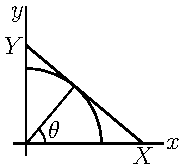
\includegraphics{minTriangle}
\end{center}

%\lower1.0in\vtop{\hsize=2.5truein \figput{minTriangle}}

This is a minimum when $\sin(2\theta)$ is a maximum. That is when
$2\theta=\dfrac{\pi}{2}$. Hence $X=\dfrac{1}{\cos(\pi/4)}$ and
$Y=\dfrac{1}{\sin(\pi/4)}$. That is, $X=Y=\sqrt{2}$.

\end{solution}



\begin{Mquestion}[2006H]
 A rectangle is inscribed in a semicircle of radius $R$
so that one side of the rectangle lies along a diameter of the semicircle.
Find the largest possible perimeter of such a rectangle, if it exists,
or explain why it does not. Do the same for the smallest possible perimeter.
\begin{center}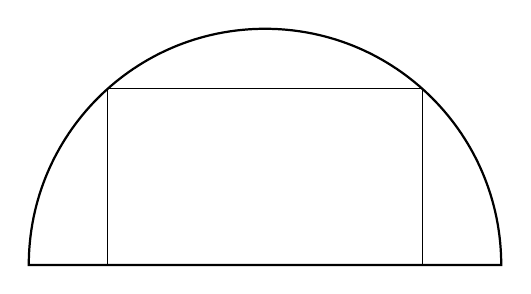
\begin{tikzpicture}
\draw[thick] (3,0) arc (0:180:3cm) --cycle;
\draw (2,0)--(2,2.24)-|(-2,0);
\end{tikzpicture}\end{center}
\end{Mquestion}
\begin{hint}
Put the whole system on $xy$-axes, so that you can easily describe the pieces using $(x,y)$-coordinates.
\end{hint}
\begin{answer}
The largest possible perimeter is $2\sqrt{5}R$ and
the smallest possible perimeter is $2R$.
\end{answer}
\begin{solution}
For ease of notation, we place the semicircle on a Cartesian plane with diameter along the $x$-axis and centre at the origin.
\begin{center}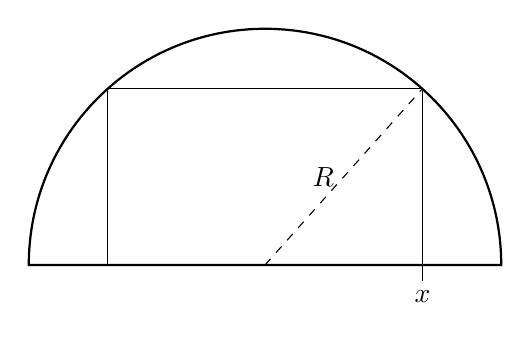
\begin{tikzpicture}
\YEaaxis{4}{4}{.5}{4}
\draw[thick] (3,0) arc (0:180:3cm) --cycle;
\draw (2,0)--(2,2.24)-|(-2,0);
\draw (2,.2)--(2,-.2) node[below]{$x$};
\draw[dashed] (0,0)--(2,2.24) node[midway, left]{$R$};
\end{tikzpicture}\end{center}
If $x$ is the point where the rectangle touches the diameter to the right of the $y$-axis, then $2x$ is the width of the rectangle. The origin and the two right corners of the rectangle form a right triangle with hypotenuse $R$, so by the Pythagorean Theorem,
the upper right hand corner
of the rectangle is at $\big(x,\sqrt{R^2-x^2}\big)$. The perimeter of the rectangle is given by the function:
\begin{align*}
P(x)&=4x+2\sqrt{R^2-x^2}
\intertext{So, this is what we optimize. The endpoints of the domain for this function are $x=0$ and $x=R$. To find the critical points, we differentiate:}
 P'(x)&=4-\dfrac{2x}{\sqrt{R^2-x^2}}\\
P'(x)=0\iff 4&=\dfrac{2x}{\sqrt{R^2-x^2}}\\
 x&=2\sqrt{R^2-x^2}\\
x^2&=4(R^2-x^2)\\
5x^2&=4R^2\\
x&=\dfrac{2}{\sqrt{5}}R
\end{align*}
Note that since our perimeter formula was defined to work only for $x$ in $[0,R]$, we neglect the negative square root, $-\dfrac{2}{\sqrt{5}}R$.

Now, we find the size of the perimeter at the critical point and the endpoints:

\begin{center}
\begin{tabular}{|c||c|c|c|}
\hline
$c$ & $0$ &  $R$ &  $\frac{2}{\sqrt{5}}R$  \\
\hline
type & endpoint & endpoint & critical point  \\
\hline
$P(c)$ & $2R$ & $4R$ & $2\sqrt{5}R$ \\
\hline
\end{tabular}
\end{center}
%$$
%P(0)=2R\qquad
%P\left(\dfrac{2}{\sqrt{5}}R\right)=2\sqrt{5}R\qquad
%P(R)=4R
%$$
So, the largest possible perimeter is $2\sqrt{5}R$ and
the smallest possible perimeter is $2R$.

Remark: as a check on the correctness of our formula for $P(x)$,
          when $x=0$ the rectangle degenerates to the line segment from
          $(0,0)$ to $(0,R)$. The perimeter of this ``width zero rectangle''
          is $2R$, agreeing with $P(0)$.
          Similarly, when $x=R$ the rectangle degenerates
          to the line segment from $(R,0)$ to $(-R,0)$. The perimeter
          of this ``width zero rectangle'' is $4R$, agreeing with $P(R)$.
\end{solution}




\begin{Mquestion}[2009H]
Find the maximal possible volume of a cylinder with surface
area $A$.\footnote{Food is often packaged in cylinders, and companies wouldn't want to waste the metal they are made out of. So, you might expect the dimensions you find in this problem to describe a tin of, say, cat food. \href{http://jerryfarlow.com/wp-content/uploads/2015/11/A24-YOU-DO-THE-CALCULUS-WE-WILL-DO-THE-CAT-FOOD.pdf}{Read here} about why this \emph{isn't} the case.}
\end{Mquestion}
\begin{hint}
The surface area consists of two discs and a
strip. Find the areas of these pieces.

The volume of a cylinder with radius $r$ and height $h$ is $\pi r^2 h$.
\begin{center}\begin{tikzpicture}
\draw (0,3) node[shape=ellipse, inner sep=0, minimum width=3cm, minimum height=1cm, draw, fill=blue, fill opacity=0.1]{};
\draw (0,0) node[shape=ellipse, inner sep=0, minimum width=3cm, minimum height=1cm, draw]{};
\draw (-1.5,0)--(-1.5,3);
\draw (1.5,0)--(1.5,3) node[midway, right]{$h$};
\draw (0,3)node[vertex]{};
\draw (0,3)--(1.5,3) node[midway, above]{$r$};
\draw[->, ultra thick, red] (3,1.5)--(4,1.5) ;
\draw (8,-1.5) node[shape=circle, minimum size=3cm, draw, inner sep=0]{};
\draw (8,4.5) node[shape=circle, minimum size=3cm, draw, inner sep=0, fill=blue, fill opacity=0.1]{};
\draw (8,4.5) node[vertex]{} -- (9.5,4.5) node[midway, above]{$r$};
\draw (5,0)--(14,0)--(14,3)node[midway, right]{$h$}--(5,3) --(5,0);
\end{tikzpicture}\end{center}
\end{hint}
\begin{answer}
$\dfrac{A^{3/2}}{3\sqrt{6\pi}}$
\end{answer}
\begin{solution} Let the cylinder have radius $r$ and height $h$. If we imagine popping off the ends, they are two circular disks, each with surface area $\pi r^2$. Then we imagine unrolling the remaining tube. It has height $h$, and its other dimension is given by the circumference of the disks, which is $2\pi r$. Then the area of the ``unrolled tube" is $2\pi rh$.
\begin{center}\begin{tikzpicture}
\draw (0,3) node[shape=ellipse, inner sep=0, minimum width=3cm, minimum height=1cm, draw, fill=blue, fill opacity=0.1]{};
\draw (0,0) node[shape=ellipse, inner sep=0, minimum width=3cm, minimum height=1cm, draw]{};
\draw (-1.5,0)--(-1.5,3);
\draw (1.5,0)--(1.5,3) node[midway, right]{$h$};
\draw (0,3)node[vertex]{};
\draw (0,3)--(1.5,3) node[midway, above]{$r$};
\draw[->, ultra thick, red] (3,1.5)--(4,1.5) ;
\draw (8,-1.5) node[shape=circle, minimum size=3cm, draw, inner sep=0]{};
\draw (8,4.5) node[shape=circle, minimum size=3cm, draw, inner sep=0, fill=blue, fill opacity=0.1]{};
\draw (8,4.5) node[vertex]{} -- (9.5,4.5) node[midway, above]{$r$};
\draw (5,0)--(14,0)--(14,3)node[midway, right]{$h$}--(5,3)  --(5,0);
\draw (9.5,1.5) node{$(2\pi r) h$};
\draw (8,-1.5) node{$\pi r^2$};
\end{tikzpicture}\end{center}
So, the surface area is $2\pi r^2+2\pi r h$. Since the area is given as $A$, we can solve for $h$:
\begin{align*}
A&=2\pi r^2+2\pi r h\\
2\pi r h &=A-2\pi r^2\\
 h&=\dfrac{A-2\pi r^2}{2\pi r}.
\end{align*}
Then we can write the volume as a function of the variable $r$ and the constant $A$:
\begin{align*}
V(r)&=\pi r^2 h\\
&=\pi r^2 \left(\dfrac{A-2\pi r^2}{2\pi r}\right)\\
&=\dfrac{1}{2}\left(Ar-2\pi r^3\right)
\intertext{This is the function we want to maximize. Let's find its critical points.}
V'(r)&=\dfrac{1}{2}\left(A-6\pi r^2\right)\\
V'(r)=0 &\iff A=6\pi r^2 \iff r=\sqrt{\dfrac{A}{6\pi}}
\intertext{since negative values of $r$ don't make sense. At this critical point,}
V\left(\sqrt{\dfrac{A}{6\pi}}\right)&=
\dfrac{1}{2}\left[A\left(\sqrt{\dfrac{A}{6\pi}}\right)-2\pi \left(\sqrt{\dfrac{A}{6\pi}}\right)^3\right]\\
&=\dfrac{1}{2}\left[\dfrac{A^{3/2}}{\sqrt{6\pi}}-\dfrac{2\pi A^{3/2}}{6\pi\sqrt{6\pi}}\right]\\
&=\dfrac{1}{2}\left[\dfrac{A^{3/2}}{\sqrt{6\pi}}-\dfrac{A^{3/2}}{3\sqrt{6\pi}}\right]\\
&=\dfrac{A^{3/2}}{3\sqrt{6\pi}}.
\end{align*}
We should also check the volume of the cylinder at the endpoints of the function. Since $r \geq 0$, one endpoint is $r=0$. Since $h \geq 0$, and $r$ grows as $h$ shrinks, the other endpoint is whatever value of $r$ causes $h$ to be 0. We could find this value of $r$, but it's not strictly necessary: when $r=0$, the volume of the cylinder is zero, and when $h=0$, the volume of the cylinder is still zero. So, the maximum volume does not occur at the endpoints.

Therefore, the maximum volume is achieved at the critical
point, where $$
V_{\rm max}=\dfrac{A^{3/2}}{3\sqrt{6\pi}}.
$$

Remark: as a check, $A$ has units $m^2$ and, because of the
         $A^{3/2}$, our answer has units $m^3$, which are the correct
         units for a volume.
\end{solution}


\begin{Mquestion}[2007H]
 What is the largest possible area of a window, with perimeter $P$,
in the shape of a rectangle with a semicircle on top (so the diameter of the
semicircle equals the width of the rectangle)?
\end{Mquestion}
\begin{hint}
If the circle has radius $r$, and the entire window has perimeter $P$, what is the height of the rectangle?
\end{hint}
\begin{answer}
$\dfrac{P^2}{2(\pi+4)}$
\end{answer}
\begin{solution}
 Denote by $r$ the radius of the semicircle, and let $h$ be the height of the rectangle. \begin{center}\begin{tikzpicture}
\draw (3,0) arc  (0:180:3);
\draw (3,0)--(3,-2)--(-3,-2)--(-3,0);
\draw[dashed] (0,0)--(3,0) node[midway, above]{$r$};
\draw (0,0) node[vertex]{};
\draw[dashed](0,0)--(0,-2) node[midway, right]{$h$};
\draw[red, <->] (3.5,0) arc  (0:180:3.5);
\draw[red] (0,3.75)node{$\pi r$};
\draw[red, <->] (3,-2.5)--(-3,-2.5) node[midway, below]{$2 r$};
\draw[blue, <->] (-3.75,0)--(-3.75,-2) node[midway, left]{$h$};
\draw[blue, <->] (3.75,0)--(3.75,-2) node[midway, right]{$h$};
\end{tikzpicture}\end{center}
Since the perimeter
is required to be $P$, the height, $h$, of the rectangle must obey
\begin{align*}
P&=\pi r+2r+2h\\
h&=\dfrac{1}{2}(P-\pi r -2r)
\end{align*}
So the area is
\begin{align*}
A(r)&=\half\pi r^2 +2rh\\
    &=\half\pi r^2 +r(P-\pi r-2r)\\
    &=rP-\half(\pi+4)r^2
    \intertext{Finding all critical points:}
0=A'(r)&=P-(\pi+4)r\\
 r&=\dfrac{P}{\pi+4}
\end{align*}

Now we want to know what radius yields the maximum area. We notice that
$A'(r)>0$ for $r<\dfrac{P}{\pi+4}$ and $A'(r)<0$ for $r>\dfrac{P}{\pi+4}$.
So, $A(r)$ is increasing until the critical point, then decreasing after it. That means
 \emph{the global maximum occurs at the critical point,}
$r=\dfrac{P}{\pi+4}$. The maximum area is
\begin{align*}
rP-\frac{1}{2}(\pi+4)r^2&=\dfrac{P^2}{\pi+4}-\frac{1}{2}(\pi+4)\dfrac{P^2}{(\pi+4)^2}\\
&=\dfrac{P^2}{2(\pi+4)}
\end{align*}

Remark: another way to see that the global maximum occurs at the critical point is to compare the area at the critical point to the areas at the endpoints of the function. The smallest value of $r$ is 0, while the biggest is $\dfrac{P}{\pi+2}$ (when the shape is simply a half-circle). Comparing $A(0)$, $A\left(\dfrac{P}{\pi+2}\right)$, and
$A\left(\dfrac{P}{\pi+4}\right)$ is somewhat laborious, but certainly possible.
\end{solution}


\begin{question}[2010H]\label{s3.5.3formulalast}
Consider an open-top rectangular baking pan with base dimensions
$x$ centimetres by $y$ centimetres and height $z$ centimetres that is
made from $A$ square centimetres of tin plate. Suppose $y = px$ for some
fixed constant $p$.
\begin{enumerate}[(a)]
\item Find the dimensions of the baking pan with the maximum
capacity (i.e., maximum volume). Prove that your answer yields the
baking pan with maximum capacity. Your answer will depend on the value of $p$.
\item Find the value of the constant $p$ that yields the baking
pan with maximum capacity and give the dimensions of the resulting
baking pan. Prove that your answer yields the baking pan with maximum
capacity.
\end{enumerate}
\end{question}
%\begin{hint}
%\end{hint}
\begin{answer}
(a)
$x=\sqrt{\dfrac{A}{3p}}$,
$y=\sqrt{\dfrac{Ap}{3}}$, and
$z=\dfrac{\sqrt{Ap}}{\sqrt{3}(1+p)}$

(b) $p=1$

(The dimensions of the resulting baking pan are
      $x=y=\sqrt{ \dfrac{A}{3} }$ and $z=\dfrac{1}{2}\sqrt{ \dfrac{A}{3} }$.)
\end{answer}
\begin{solution}
\begin{center}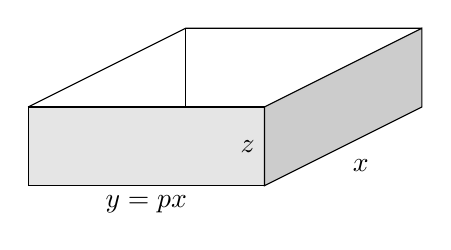
\begin{tikzpicture}
\draw[fill=black, fill opacity=0.1] (0,0)--(3,0)--(3,1)--(0,1)--cycle;
\draw[fill=black, fill opacity=0.2] (3,0)--(3,1)--(5,2)--(5,1)--cycle;
\draw (5,2)--(2,2)--(0,1);
\draw (2,2)--(2,1);
\draw (1.5,0) node[below]{$y=px$};
\draw (4,0.25) node[right]{$x$};
\draw (3,.5) node[left]{$z$};
\end{tikzpicture}\end{center}
(a) The surface area of the pan is
\begin{align*}
xy+2xz+2yz&=px^2+2xz+2pxz\\
&=px^2+2(1+p)xz
\end{align*}
and the volume of the pan is $xyz=px^2z$. Assuming that all $A\,{\rm cm}^2$
is used, we have the constraint
$$
px^2+2(1+p)xz=A \qquad\hbox{or}\quad z=\dfrac{A-px^2}{2(1+p)x}
$$
So
\begin{align*}
V(x)&=xyz=x(px)\left(\frac{A-px^2}{2(1+p)x}\right)
\\&=\dfrac{p}{2(1+p)}x(A-px^2)\intertext{Using the product rule,}
  V'(x)&=\dfrac{p}{2(1+p)}\left[x(-2px)+(A-px^2)\right]\\
  &=\dfrac{p}{2(1+p)}\big[A-3px^2\big]
\end{align*}
The derivative $V'(x)$ is 0 when $x=\sqrt{\dfrac{A}{3p}}$. The derivative
is positive (i.e. $V(x)$ is increasing) for $x< \sqrt{\dfrac{A}{3p}}$ and
is negative (i.e. $V(x)$ is decreasing) for $x>\sqrt{\dfrac{A}{3p}}$. So
the pan of maximum volume has dimensions $x=\sqrt{\dfrac{A}{3p}}$,
$y=p\sqrt{\dfrac{A}{3p}}=\sqrt{\dfrac{Ap}{3}}$ and
$z=\dfrac{2A/3}{2(1+p)\sqrt{A/(3p)}}=\dfrac{\sqrt{Ap}}{\sqrt{3}(1+p)}$.
\item{}(b) The volume of the pan from part (a) is
$$
V(p)=\left(\sqrt{\dfrac{A}{3p}}\right)\left(p\sqrt{\dfrac{A}{3p}}\right)
\dfrac{\sqrt{Ap}}{\sqrt{3}(1+p)}
=\left(\dfrac{A}{3}\right)^{3/2}\dfrac{\sqrt{p}}{1+p}
$$
Since
$$
\diff{}{p}\left\{\dfrac{\sqrt{p}}{1+p}\right\}=\dfrac{\half (1+p)/\sqrt{p}-\sqrt{p}}{(1+p)^2}
=\dfrac{\sqrt{p}\left(\dfrac{1}{p}-1\right)}{2(1+p)^2}
$$
the volume is increasing with $p$ for $p<1$ and decreasing with $p$ for
$p>1$. So the maximum volume is achieved for $p=1$ (a square base).
\end{solution}




%%%%%%%%%%%%%%%%%%
\subsection*{\Application}
%%%%%%%%%%%%%%%%%%
\begin{Mquestion}[1999H]
Let $f(x)=x^x$ for $x>0$.\begin{enumerate}[(a)]
\item\label{s2.10xx1} Find $f'(x)$.
\item\label{s2.10xx2} At what value of $x$ does the curve $y=f(x)$ have a horizontal
tangent line?
\item\label{s2.10xx3} Does the function $f$ have a local maximum, a local minimum,
or neither of these at the point $x$ found in part \eqref{s2.10xx2}?
\end{enumerate}
\end{Mquestion}
\begin{hint} Use logarithmic differentiation to find $f'(x)$.
\end{hint}
\begin{answer}
\eqref{s2.10xx1} $x^x(1+\log x)$
\qquad \eqref{s2.10xx2} $x=\dfrac{1}{e}$
\qquad \eqref{s2.10xx3} local minimum
\end{answer}
\begin{solution}
\eqref{s2.10xx1} We use logarithmic differentiation.
\begin{align*}
f(x)&=x^x\\
\log f(x)&=\log \left(x^x\right)=x\log x\\
\diff{}{x}\left\{\log f(x)\right\}&=\diff{}{x}\left\{x\log x\right\}\\
\frac{f'(x)}{f(x)}&=x\left(\frac{1}{x}\right)+\log x=1+\log x\\
f'(x)&=f(x)\left(1+\log x\right)=x^x(1+\log x)
\end{align*}

\eqref{s2.10xx2} Since $x>0$, $x^x>0$. Therefore,
\[f'(x)=0\iff 1+\log x=0\iff \log x=-1\iff x=\dfrac{1}{e}\]

\eqref{s2.10xx3}
 Since $x>0$, $x^x>0$. So, the sign of $f'(x)$ is the same as the sign of $1+\log x$.

 For $x<\dfrac{1}{e}$, $\log x<-1$ and $f'(x)<0$. That is, $f(x)$
decreases as $x$ increases, when $x<\dfrac{1}{e}$.
For $x>\dfrac{1}{e}$, $\log x>-1$ and $f'(x)>0$.  That is, $f(x)$
increases as $x$ increases, when $x>\dfrac{1}{e}$. Hence $f(x)$
is a {local minimum} at $x=\dfrac{1}{e}$.
\end{solution}


\begin{Mquestion}[2011H]
A length of wire is cut into two pieces, one of which is bent
to form a circle, the other to form a square. How should the wire be cut
if the area enclosed by the two curves is maximized?
How should the wire be cut
if the area enclosed by the two curves is minimized? Justify your answers.
\end{Mquestion}
\begin{hint}
When you are finding the global extrema of a function, remember to check endpoints as well as critical points.
\end{hint}
\begin{answer}
Maximum area: do not cut, make a circle and no square.\\ Minimum area: make a square out of a piece that is $\dfrac{4}{4+\pi}$ of the total length of the wire.
\end{answer}
\begin{solution}
Call the length of the wire $L$ units and suppose that it
is cut $\ell$ units from one end. Make the square from the piece of length $\ell$, and make the circle from the remaining piece of length $L-\ell$.

The square has perimeter $\ell$, so its side length is $\ell/4$
and its area is $\left(\dfrac{\ell}{4}\right)^2$.
The circle has circumference $L-\ell$, so its radius is
$\dfrac{L-\ell}{2\pi}$ and its area is $\pi\left(\dfrac{L-\ell}{2\pi}\right)^2=\dfrac{(L-\ell)^2}{4\pi}$.

The area enclosed by the shapes, when the square is made from a length of size $\ell$, is
\begin{align*}
A(\ell)&=\dfrac{\ell^2}{16}+\dfrac{(L-\ell)^2}{4\pi}
\intertext{We want to find the global max and min for this function, given the constraint $0 \leq \ell \leq L$, so we find its derivative:}
A'(\ell)&=\dfrac{\ell}{8} -\dfrac{L-\ell}{2\pi}
         =\dfrac{\pi+4}{8\pi}\ell-\dfrac{L}{2\pi}
\intertext{Now, we find the critical point.}
A'(\ell)&=0\\
\frac{\pi+4}{8\pi}\ell&=\frac{L}{2\pi}\\
\ell&=\frac{4L}{\pi+4}
\end{align*}
\begin{center}
\begin{tabular}{|c||c|c|c|}
\hline
$\ell$ & $0$ &  $L$ &  $\textcolor{white}{\dfrac{.^.}{.}}\frac{4L}{\pi+4}$  \\
\hline
type & endpoint & endpoint & critical point  \\
\hline
$A(\ell)$ & $\textcolor{white}{\dfrac{.^.}{.}}\frac{L^2}{4\pi}$ & $\frac{L^2}{16}_{}$ & $A\left(\frac{4L}{\pi+4}\right)$ \\
\hline
\end{tabular}
\end{center}
 It seems obnoxious to evaluate $A\left(\frac{4L}{\pi+4}\right)$, and the problem doesn't ask for it--but we still have to figure out whether it is a global max or min.

 When $\ell<\frac{4L}{\pi+4}$, $A'(\ell)<0$, and when
 $\ell>\frac{4L}{\pi+4}$, $A'(\ell)>0$. So, $A(\ell)$ is decreasing until $\ell=\frac{4L}{\pi+4}$, then increasing. That means our critical point $\ell=\frac{4L}{\pi+4}$
 is a local minimum.

So, the minimum occurs at the only critical point, which is $\ell=\left(\dfrac{4}{4+\pi}\right)L$. This corresponds to $\dfrac{\ell}{L}=\dfrac{4}{4+\pi}$: the proportion of the wire that is cut is $\dfrac{4}{4+\pi}$.

The maximum has to be either at $\ell=0$ or at $\ell=L$.
As $A(0)=\dfrac{L^2}{4\pi} > A(L)=\dfrac{L^2}{16}$, the maximum has $\ell=0$
(that is, no square).
\end{solution}




%this is done in notes
%\begin{question}[1997A]
%A rectangular sheet of cardboard is 6 inches by 9 inches. Four
%identical squares are cut from the corners of the cardboard as shown in
%the figure and the remaining piece is folded into an open rectangular box.
%What should the size of the cut out squares be in order to maximize the
%volume of the box?
%\begin{center}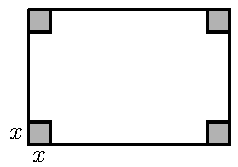
\includegraphics{box}\end{center}
%\end{question}
%\begin{answer}$x=\dfrac{5-\sqrt{7}}{2}\approx 1.18$
%\end{answer}
%\begin{solution} The box has height $x$ and base $(6-2x)\times(9-2x)$.
%So the box has volume $x(6-2x)(9-2x)=54x-30x^2+4x^3$. This volume is a maximum %when
%$$
%0=\diff{}{x}(54x-30x^2+4x^3)=54-60x+12 x^2
%=6(9-10x+2x^2)
%\implies x=\dfrac{10\pm\sqrt{100-4\times2\times 9}}{4}
%$$
%Since $x$ runs from 0 to 3 (at which point the short dimension of the base has
%shrunk to zero) and both $x=0$ and $x=3$ give volume zero, the maximum
%must be achieved by one of $\dfrac{10\pm\sqrt{100-72}}{4}
%=\dfrac{10\pm\sqrt{28}}{4}=\dfrac{10\pm2\sqrt{7}}{4}
%=\dfrac{5\pm\sqrt{7}}{2}$. The plus sign,
%$\dfrac{5+\sqrt{7}}{2}\approx 3.8$ is outside the allowed range for $x$,
%the maximum is given by \boxed{x=\dfrac{5-\sqrt{7}}{2}\approx 1.18}$\,$.
%\end{solution}
